\section{Durchführung}
Das Experiment besteht dann darin den Photostrom in Abhängigkeit der angelegten Spannung zu messen.
Dazu wird die in Abbildung \ref{fig:aufbau3} gezeigte Schaltung verwendet.

\begin{figure}[h]
    \centering
    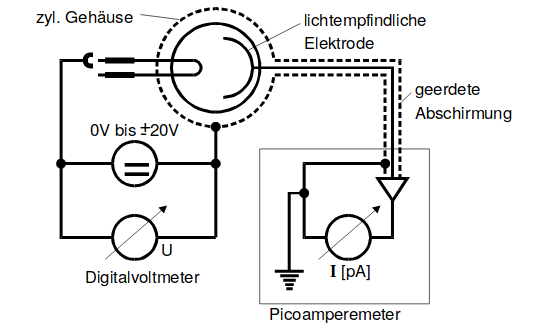
\includegraphics[height=5cm]{Durchführung/Aufbau3.png}
    \caption{.Schaltung zur Messung des Photostroms}
    \label{fig:aufbau3}
\end{figure}

Zunächst wird die Grenzspannung $U_\text{g}$ gesucht, bei der der Photostrom verschwindet.
Dann werden die paarigen Messwerte für die eingestellte Gegenspannung $U_\text{geg}$ und den gemessenen Photostrom $I_\text{Photo}$ aufgezeichnet.
Hierbei sollten für vier verschiedene Spektrallinien jeweils 10 Messwerte notiert werden.
Außerdem sollen für die orangene Spektrallinie 20 Messwerte aufgenommen werden.
Es sollte beachtet werden, dass in dem Intervall $U_\text{geg} \in [0,U_g]$ gemessen wird.
Zusätzlich dazu sollen bei der orangenen Spektrallinie jeweils 5 Messwerte im Bereich $U_\text{geg} < 0$, also mit einer Beschleungigungsspannung $U_b$, und im Bereich $U_\text{geg} > U_g$ gemessen werden.
